% !TeX spellcheck = en_AU
% !TeX program = pdflatex
%
% LuxSleek-CV 1.1 LaTeX template
% Author: Andreï V. Kostyrka, University of Luxembourg
%
% 1.1: added tracking and letter-spacing for prettier lower caps, added `~` for language levels
% 1.0: initial release

\documentclass[11pt, a4paper]{article} 

\usepackage[T1]{fontenc}     % We are using pdfLaTeX,
\usepackage[utf8]{inputenc}  % hence this preparation
\usepackage[british]{babel}  
\usepackage[left = 0mm, right = 0mm, top = 0mm, bottom = 0mm]{geometry}
\usepackage[stretch = 25, shrink = 25, tracking=true, letterspace=30]{microtype}  
\usepackage{graphicx}        % To insert pictures
\usepackage{xcolor}          % To add colour to the document
\usepackage{marvosym}        % Provides icons for the contact details

\usepackage{enumitem}        % To redefine spacing in lists
\setlist{parsep = 0pt, topsep = 0pt, partopsep = 1pt, itemsep = 1pt, leftmargin = 6mm}

\usepackage{FiraSans}        % Change this to use any font, but keep it simple
\renewcommand{\familydefault}{\sfdefault}

\definecolor{cvblue}{HTML}{304263}

%%%%%%% USER COMMAND DEFINITIONS %%%%%%%%%%%%%%%%%%%%%%%%%%%
% These are the real workhorses of this template
\newcommand{\dates}[1]{\hfill\mbox{\textbf{#1}}} % Bold stuff that doesn’t got broken into lines
\newcommand{\is}{\par\vskip.5ex plus .4ex} % Item spacing
\newcommand{\smaller}[1]{{\small$\diamond$\ #1}}
\newcommand{\headleft}[1]{\vspace*{3ex}\textsc{\textbf{#1}}\par%
    \vspace*{-1.5ex}\hrulefill\par\vspace*{0.7ex}}
\newcommand{\headright}[1]{\vspace*{2.5ex}\textsc{\Large\color{cvblue}#1}\par%
     \vspace*{-2ex}{\color{cvblue}\hrulefill}\par}
%%%%%%%%%%%%%%%%%%%%%%%%%%%%%%%%%%%%%%%%%%%%%%%%%%%%%%%%%%%%

\usepackage[colorlinks = true, urlcolor = white, linkcolor = white]{hyperref}

\begin{document}

% Style definitions -- killing the unnecessary space and adding the skips explicitly
\setlength{\topskip}{0pt}
\setlength{\parindent}{0pt}
\setlength{\parskip}{0pt}
\setlength{\fboxsep}{0pt}
\pagestyle{empty}
\raggedbottom

\begin{minipage}[t]{0.33\textwidth} %% Left column -- outer definition
%  Left column -- top dark rectangle
\colorbox{cvblue}{\begin{minipage}[t][5mm][t]{\textwidth}\null\hfill\null\end{minipage}}

\vspace{-.2ex} % Eliminates the small gap
\colorbox{cvblue!90}{\color{white}  %% LEFT BOX
\kern0.09\textwidth\relax% Left margin provided explicitly
\begin{minipage}[t][293mm][t]{0.82\textwidth}
\raggedright
\vspace*{2.5ex}

\Large Samuel \textbf{\textsc{Marks}}, PhD \normalsize 

% Centering without extra vertical spacing
\null\hfill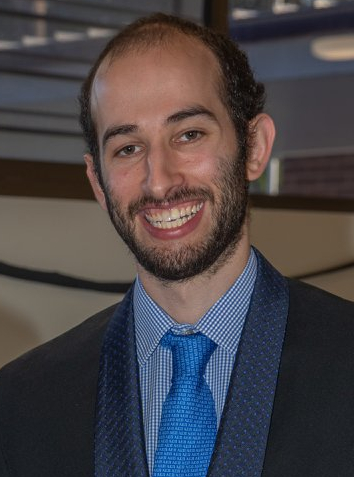
\includegraphics[width=0.65\textwidth]{user.jpg}\hfill\null

\vspace*{0.5ex} % Extra space after the picture

\headleft{Modus Operandi}
Split my life in three: family; medical charity; and business. The unrelated-to-medicine business funds the first two. Focus is on open-source scalable engineering. Recently awarded an in-kind \textbf{grant worth \$3.2M} for neural compute processor access from Google.

\headleft{Links}
\small % To fit more content
\MVAt\ \href{mailto://simarks@meei.harvard.edu}{\small simarks@meei.harvard.edu} \\[0.4ex]
\Mundus\ \href{https://github.com/SamuelMarks}{github.com/SamuelMarks} \\[0.1ex]
\normalsize

\headleft{Career cliff notes}
\smaller{As a contractor working on unrelated sensor network metric aggregation, showed the largest communications company in Australia how to \textbf{save \$100M;}}\\
%   \item As a full-time employee at 16/17 years old, showed a large Travel
% company how to reduce staff count by 8 (making myself and my
% tech support department redundant);
\smaller{Given the entire top floor of the JP Morgan building to go from nothing to a full product in the Natural Language Processing (NLP) industry (all my subcontractors, including postdoctoral computational linguists)… with the backing of a billionaire family. Company \textbf{acquired by calendly};}\\
\smaller{Built a stock market analytics platform (for a high-net-worth individual);}\\
\smaller{Created deduplication algorithms and databases for helping one large bank\textemdash{}who bought another large bank\textemdash{}to join customer profiles (for a Venture Capital fund, who then proceeded to \textbf{raise \$60M} off this);}\\
\smaller{Engineered a distributed system for a blockchain company (my ‘stock’ in their company has since \textbf{gone up > 16000\%}).}

\end{minipage}%
\kern0.09\textwidth\relax%%Right margin provided explicitly to stretch the colourbox
}
\end{minipage}% Right column
\hskip2.5em% Left margin for the white area
\begin{minipage}[t]{0.56\textwidth}
\setlength{\parskip}{0.8ex}% Adds spaces between paragraphs; use \\ to add new lines without this space. Shrink this amount to fit more data vertically

\vspace{2ex}
\hypersetup{urlcolor=black}
\hypersetup{linkcolor=black}
\headright{Experience}

\textit{Mass. Eye and Ear Infimary / Harvard Medical School.}  \dates{2021+} \\
\smaller{Collaborating with ophthalmologists on initiating new medical diagnostic screening programmes that are wholly charitable, open-source, patent-free, and AI-driven; and analysing \& modelling from historical data in preparation.}

\is
\textsc{Director} at \textit{Sydney Scientific.} \dates{2015+} \\
\smaller{Engineering software for high-net-worth individuals, small companies, and venture capitalists. Open-source focus, creating compilers and distributed systems to scale from 1 user, 1 developer, and 1 device to millions of users, thousands of developers, and ten thousand servers.\\\textit{NOTE: Firm purposefully avoids anything related to medicine so as to avoid actual\textemdash{}or perceived\textemdash{}conflicts of interest with charitable research.}} 


\headright{Education}

\textsc{Fellowship}. \textit{Harvard Medical School}. \dates{2021+} \\
\smaller{Here in Cambridge MA:\begin{itemize}
  \item to analyse historical records to develop open-source predictive and interpretive models; and to
  \item initiate new medical diagnostic screening programmes; analyse \& learn from its results; and, perpetually
  \item to run better, bigger screening programmes.
\end{itemize}
I am working with Professor David Friedman (Director of Glaucoma and Medical Director for Clinical Research and Co-Director of the Glaucoma Center of Excellence).
All research is wholly charitable, open-source, and patent-free\ldots{} with a view towards global screening (self-funded through my consultancy).}

\textsc{Doctor of Philosophy} (Medicine). \textit{University of Sydney}. \dates{2015--2020} \\
\smaller{Thesis title: \textit{Facilitating large-scale glaucoma and diabetic retinopathy screening using novel technologies.}} \\
\smaller{Created technologies to facilitate mass-screening for blinding eye diseases glaucoma and diabetic retinopathy (DR). Namely:
\begin{itemize}
  \item State of the Art \textbf{(SOTA) ML} results for differentiating glaucoma from nonglaucoma using the landmark Blue Mountains Eye Study (BMES) and REFUGE fundus photo datasets
  \item \textbf{SOTA ML} for differentiating DR from healthy on Singapore (GON) and a new dataset we collected (DR SPOC)
  \item \textbf{SOTA ML} for determining whether images are gradable on said new dataset\(\uparrow\)
  \item 7 new smartphone ophthalmoscope designs; compared to the industry (\$6307--\$487); the last two of which were \textbf{under 1¢ [<\$0.01]} each.
  \item eLearning MOOCs to teach the basics of ophthalmoscopy and fundus photo diagnostic interpretation to medical students
  \item Glaucoma risk calculator (online, interactive, with analytics dashboard)
\end{itemize}

Led to an ophthalmologist colleague's PhD \href{https://hdl.handle.net/2123/29364}{hdl.handle.net/2123/29364} and an invitation to continue my research at Harvard Medical School / MEEI.}

\is
\textsc{Bachelor of Science}. School of Computing. \textit{Macquarie U}.  \dates{2010--2014} \\
\smaller{This degree was in a wide range of subjects that supported my passion for computer science.}


\headright{Open-source}

685+ repositories on GitHub, >300 of these original projects (not forks). Top-10 contributor to Google's Keras (14 million downloads per month, as of August 2024).

\end{minipage}

\end{document}